\section{Further biological mechanisms: a separate experiment}
\label{sec:v4}
The preceding study found small default biological effects that were not robust
across diagnostics. We therefore examined mechanisms that change decision timing
and commitment, retaining the physical simulator and the economic evaluator.
This second experiment uses new world seeds and a shorter, explicitly separate
benchmark. Its absolute coverage values must not be pooled with the earlier
one-hour benchmark.

\subsection{Literature assessment and scope of transfer}
Amichay et al.\ experimentally identified out-of-phase burst timing in juvenile
zebrafish and tested reciprocal temporal coupling in virtual reality. Within a
responsive interval, their phase response is approximated by $T=2\tau$, where
$\tau$ is the lag between a focal burst and its partner's burst~\cite{amichay2024}.
We transfer this timing relation to eligibility for changing a vessel's goal.
The seconds-to-minutes rescaling and pairing of vessel identifiers are engineering
choices, not fitted biological parameters. No hydrodynamic swimming-efficiency
benefit is assumed.

March-Pons et al.\ model threshold-dependent cross-inhibition in honeybee-inspired
decisions~\cite{marchpons2025}. Stronger consensus can trade against choosing the
better option, making benefit in a changing monitoring mission uncertain.
Our adaptation keeps persistent support for ten movement-proposal families.
These are virtual populations inside the coordinator, not ten boats or a
simulation of messages exchanged by biological scouts.

The novelty search also identified cross-inhibition in robot swarms under
biased information~\cite{zakir2026} and a revised 2026 preprint using multi-agent
reinforcement learning to study electric-fish sensing and communication
\cite{singh2026}. These are explicit adjacent precedents. Electrical signal
borrowing is modality-specific: our radar/camera abstraction contains no
corresponding emitter--receiver interaction. We did not insert a free sensor-range
multiplier or claim to have tested that phenomenon. Finding no exact match in this
bounded search would not establish priority over all USV or drone literature.

\subsection{Reciprocal handover eligibility}
Vessels are paired as $(0,1),(2,3),\ldots$ before the mission. A pair becomes
eligible for a fresh excursion only when both cached positions are within
$35$ m of their previously issued goals. At most one member of an eligible pair
can receive a changed goal. The \emph{periodic} comparator alternates eligible
identities each 60-s decision; the \emph{greedy} comparator chooses the member
with the larger coverage-gradient norm. Both share the same settling gate.

For the reciprocal rule, let $b_i$ denote the last accepted goal-change time,
and $d_i$ the next eligible time. Among due members of a settled pair, the oldest
due time wins. When a goal change for $i$ is accepted at time $t$,
\begin{align}
 b_i &\leftarrow t, &d_i&\leftarrow t+120\ \mathrm{s},\\
 \tau_{ji}&=t-b_j, &d_j&\leftarrow b_j+2\tau_{ji}
 \quad\text{if }60\leq\tau_{ji}\leq240\ \mathrm{s}.
\end{align}
Outside this interval, $d_j$ is unchanged. Initially the even/odd members have
$(b_i,d_i)=(-120,0)$ and $(-60,60)$ s, respectively. The relation reproduces
alternating eligible times in an undisturbed two-agent example; it is not a
stability result under delays. Events here are accepted coordinator decisions,
not confirmed physical motion. Cached poses, delayed commands and independent
onboard avoidance preclude a hard guarantee that only one vessel physically
moves in each pair. The simulator does not add a new acknowledgement channel.

All three handover policies use the same ten proposal slots, gradient evaluations,
energy price and acceptance threshold. Ineligible vessels retain their old goals
in every slot, including the stopping proposal. Comparison against unrestricted
economic control measures the whole restriction; reciprocal versus periodic or
greedy handover isolates the timing rule more closely.

\subsection{Nonlinear commitment to movement proposals}
For proposal $a\in\{0,\ldots,9\}$, let $J_a$ be the economic score and
$f_a\geq0$ its virtual committed fraction. A bounded quality input and its
normalized discovery preference are
\begin{align}
 z_a&=\operatorname{clip}((J_a-\max_bJ_b)/0.01,-30,0),\\
 \pi_a&=\frac{e^{z_a}}{\sum_b e^{z_b}},\qquad r_a=\frac{1}{1+4\pi_a},\\
 f_0^{\rm free}&=1-\sum_a f_a.
\end{align}
The subscript zero on $f_0^{\rm free}$ denotes the uncommitted population,
distinct from the committed fraction for proposal index zero. We integrate
\begin{equation}
 \dot f_a=f_0^{\rm free}\bigl[0.5\pi_a+0.5f_a\bigr]
 -r_af_a-f_a\sum_{b\ne a}\sigma(f_b).
\end{equation}
The linear comparator uses $\sigma(x)=x$; the nonlinear rule uses the
linearly bounded sigmoid $\sigma(x)=x/[1+e^{-10(x-0.3)}]$.
The latter response comes from Ref.~\cite{marchpons2025}; the quality mapping,
ten changing proposal families and time scale are our engineering adaptation.
Support starts at zero and persists across decisions. Each decision integrates
two dimensionless time units in 100 explicit Euler steps. Because inflows are
nonnegative on a zero component and total committed outflow returns to the
uncommitted compartment, the continuous dynamics preserve the probability
simplex. The implementation verifies simplex membership without clipping, and
a half-step check tests numerical sensitivity.

The largest committed fraction proposes the action, which is executed only if
its current modeled gain exceeds the same economic improvement threshold.
Persistence attaches to a proposal's \emph{type}, not a fixed geographic location;
changes in proposal geometry are a limitation of this memory. Unchanged sensing,
network and plant models prevent a biology-specific physical advantage by
construction. No distributed consensus or closed-loop coverage theorem is claimed.

\subsection{Frozen evaluation and computational cost}
The new nominal and short-radio profiles each use six vessels, 2400-s missions,
32 angular quadrature points on each of three annuli, and 20 secondary reference
events. The moving priority completes $2/3$ of a revolution per mission, preserving
the earlier angular speed rather than accelerating the front when shortening
the episode. Four scenarios are storm, sensor fault, moving priority and
intermittent conditions. Twelve common world-seed blocks per profile yield
576 main missions across six policies. A 12-mission integration pilot precedes
the freeze and does not select parameters.

Additional diagnostics use a probit physical detector, longer correlated
disturbances and short radio (96 missions, four seeds), and 128 planner paths
(48 missions, four seeds and two scenarios). These remain small diagnostics.
The three declared biological coverage contrasts are reciprocal minus periodic,
reciprocal minus greedy, and nonlinear minus linear inhibition. Bootstrap
intervals resample whole world-seed blocks after averaging the eight main cells;
three pooled coverage tests receive Holm correction. Energy, lower-tail coverage,
AoI, connected-graph frequency and computation are reported separately.

Each unrestricted decision uses $4N$ finite-difference field evaluations and
up to $3K$ trajectory-field evaluations for $K=10$ proposals, plus inexpensive
motion and energy forecasts. Each field evaluation samples $S$ paths over $L$
deadline rounds and $Q$ monitoring locations. Its principal scaling is
$O(SL(N^2+NQ)+N^3)$, including correlated visibility and temporal reachability;
this is not linear scaling in swarm size. The commitment update adds
$O(RK)$ work for $R=100$ internal steps. Equal proposal counts help attribution;
the settling restrictions can nevertheless generate duplicate proposals.
Wall times are measured on a shared CPU host, not as isolated hardware benchmarks.

\subsection{Results of the new mechanism tests}
The second study adds 732 model-based missions, including the pilot and declared diagnostics. Reciprocal versus periodic handover changes coverage by -0.21 [-0.35, -0.09] percentage points and total energy by -5.55 Wh. Relative to greedy handover the coverage contrast is -0.45 [-0.63, -0.28] points. Nonlinear versus linear inhibition changes coverage by +0.01 [-0.04, +0.06] points and energy by -1.48 Wh. Brackets are paired 95\% bootstrap intervals, not predictive bounds for a new vessel platform.
\begin{table}[t]\centering\small
\caption{New main-study means. Each policy has 96 missions across two radio profiles and four scenarios.}
\begin{tabular}{lrrr}\toprule Policy & $\bar C$ & $E$ [Wh] & AoI [s]\\\midrule
Economic & 0.6957 & 300.9 & 49.3 \\
Periodic handover & 0.6843 & 280.1 & 51.0 \\
Greedy handover & 0.6867 & 282.9 & 50.6 \\
Reciprocal handover & 0.6822 & 274.5 & 51.2 \\
Linear inhibition & 0.6962 & 301.0 & 49.4 \\
Nonlinear inhibition & 0.6963 & 299.5 & 49.3 \\
\bottomrule\end{tabular}\label{tab:v4means}\end{table}
\begin{figure*}[tbp]\centering
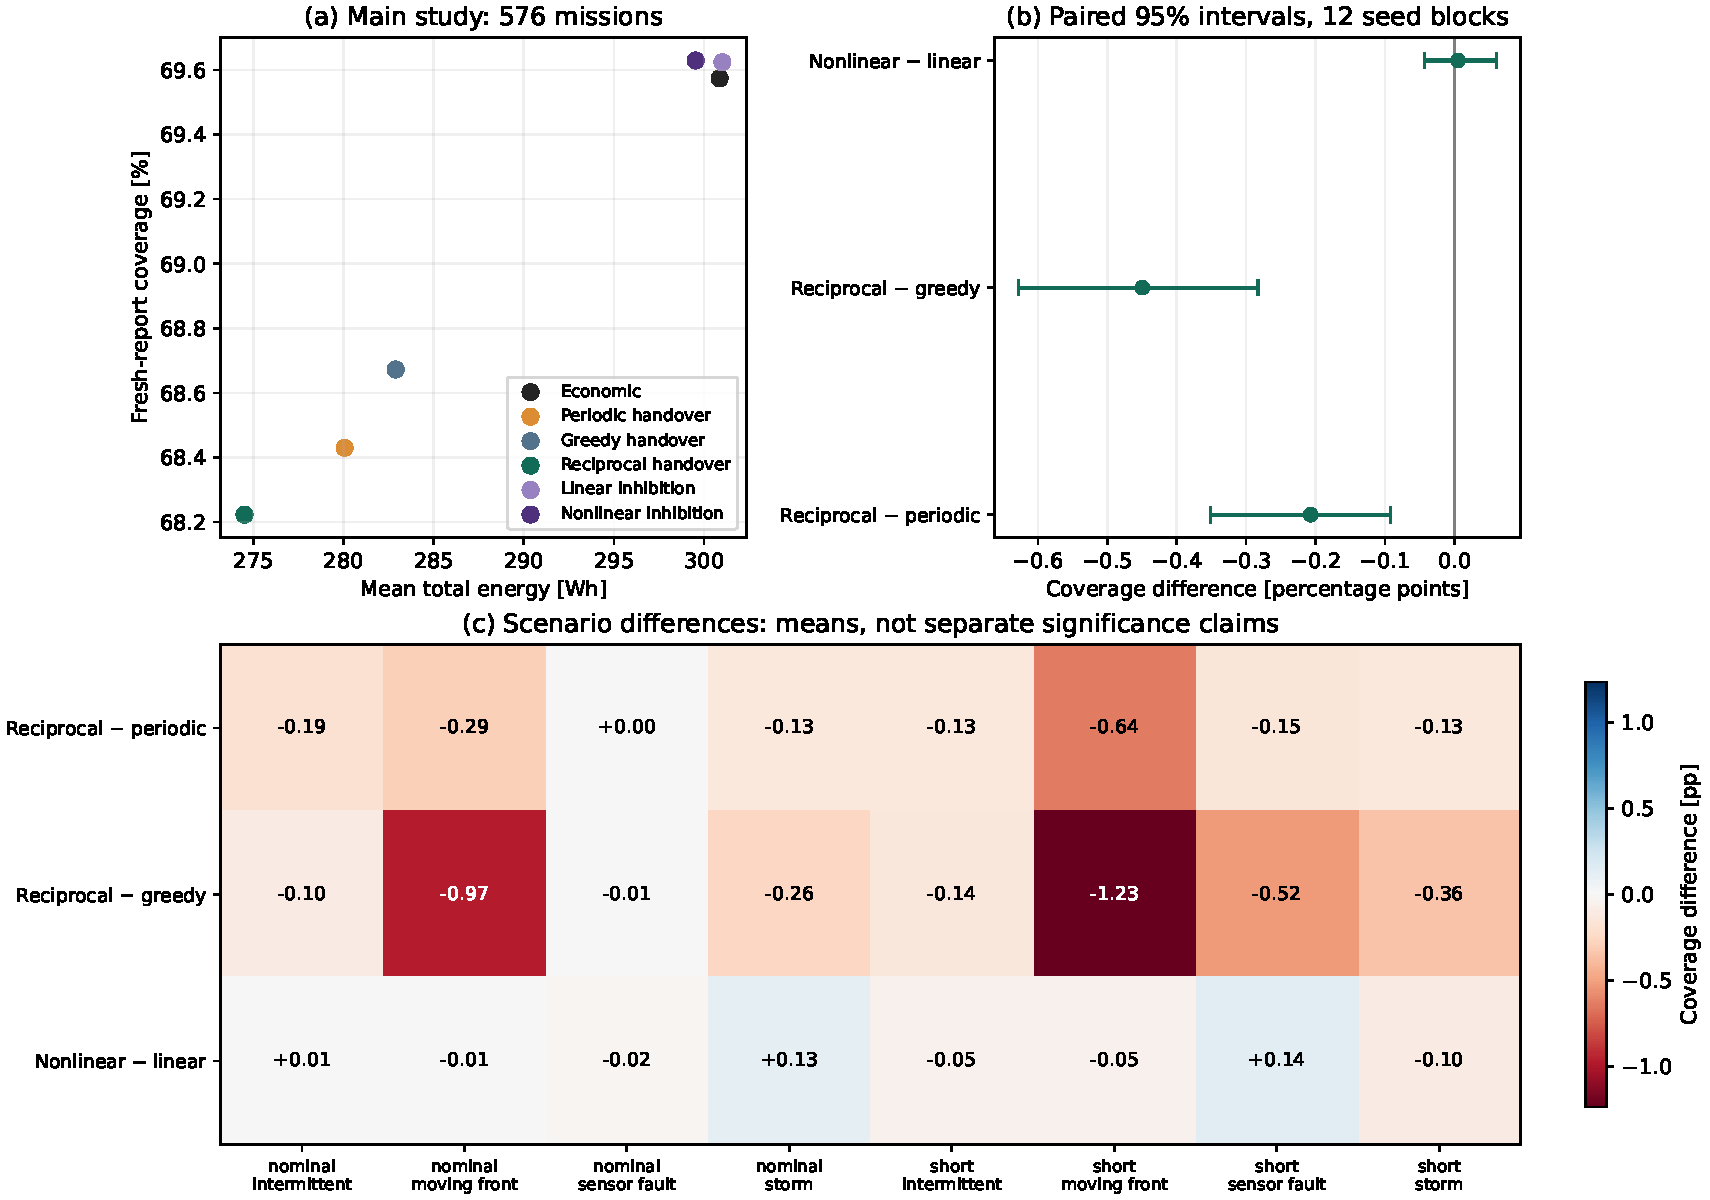
\includegraphics[width=.97\textwidth]{figures/bio_mechanisms.pdf}
\caption{Additional biological mechanisms with matched restrictions. Main-study coverage--energy means, paired coverage contrasts, and scenario-specific differences. A reduced movement budget can save energy while losing timely monitoring.}
\label{fig:v4bio}\end{figure*}
\begin{table*}[tbp]\centering\small
\caption{Prespecified new biological contrasts and small diagnostics. Coverage differences are in percentage points, with paired 95\% intervals. Main $p_H$ values apply Holm adjustment to three coverage tests; diagnostics are descriptive.}
\begin{tabular}{llrrr}\toprule Setting & Contrast & $\Delta C$ [95\% interval] & $\Delta E$ [Wh] & $p_H$\\\midrule
Main, 12 blocks & Reciprocal -- periodic & -0.21 [-0.35, -0.09] & -5.55 & 0.008 \\
Main, 12 blocks & Reciprocal -- greedy & -0.45 [-0.63, -0.28] & -8.38 & 0.002 \\
Main, 12 blocks & Nonlinear -- linear & +0.01 [-0.04, +0.06] & -1.48 & 0.850 \\
Shifted, 4 blocks & Reciprocal -- periodic & -0.28 [-0.59, +0.04] & -3.28 & -- \\
Shifted, 4 blocks & Reciprocal -- greedy & -0.36 [-0.67, -0.16] & -5.35 & -- \\
Shifted, 4 blocks & Nonlinear -- linear & -0.07 [-0.14, -0.00] & +0.46 & -- \\
128 paths, 4 blocks & Reciprocal -- periodic & +0.03 [-0.41, +0.47] & -6.16 & -- \\
128 paths, 4 blocks & Reciprocal -- greedy & -0.58 [-0.74, -0.42] & -6.32 & -- \\
128 paths, 4 blocks & Nonlinear -- linear & -0.01 [-0.21, +0.18] & +0.33 & -- \\
\bottomrule\end{tabular}\label{tab:v4contrasts}\end{table*}
These adaptations should be judged against their matched controls and against unrestricted economic control. Reciprocal handover versus economic control changes coverage by -1.35 [-1.60, -1.13] points; nonlinear inhibition versus economic control changes it by +0.06 [-0.03, +0.16] points. A small main-study contrast alone does not establish a generally useful biological advantage. The changed observation law and integration resolution are particularly relevant because all policies still optimize a sampled, imperfect prospective score.


\subsection{Why a biological transfer may not help here}
The simulator allows sensing throughout motion; it has no fitted motion-induced
sensor-blind interval. Moreover, the coordinator already computes all ten
prospective scores. Temporal alternation therefore incurs a mobility restriction
without necessarily gaining the sensory-processing advantage that motivates it
in fish. Virtual consensus does not acquire independent local evidence that
the centralized argmax comparator lacks. These are properties of the engineering
mapping, not evidence against the biological findings.

A post-hoc inspection of the eight presaved nonlinear-inhibition main missions (world seed 17000, two profiles and four scenarios) found that only 1.29\% of 310 nonstale decisions had any proposal fraction above the 0.3 sigmoid midpoint; mean maximum support was 0.091. The threshold was borrowed from a primarily binary-choice biological model, whereas these ten often similar movement proposals fragment support. This is a descriptive diagnosis, not a causal ablation: lower thresholds or grouping proposals into meaningful alternatives require a separate development and test experiment.


This suggests testing the placement of a mechanism before expanding its
complexity: a distributed information bottleneck, calibrated sensing interruption
or explicit decision-consensus requirement would have to be represented and
costed. Adding such a feature solely to favor the biological method would be
invalid. A new application model needs independent justification and new matched
controls. The current negative results should remain part of that record.

\subsection{Reinforcement learning: what is learned and how it is compared}
The executable learner selects one of nine pairs of movement step
$\{60,120,180\}$ m and economic price $\{0.0125,0.025,0.05\}$ at 60-s intervals.
It does not learn navigation, collision avoidance, task allocation or sensing
physics. Action 4 exactly recovers the standard economic controller.
Four cached observation frames feed the unchanged PPO adapter. Domain
randomization varies radio/sensor nominal ranges and mission scenarios; no true
hidden sensor health is supplied to the policy.

Three independent training seeds receive 2048 steps each, still a short pilot.
For comparison, all nine constant settings are evaluated on three separate
development world seeds in four scenarios, and the setting with the highest
mean undiscounted step reward is fixed. Every trained seed, that selected setting
and neutral action 4 are then compared on eight new world seeds. We report
discounted return, mean step reward, post-warmup coverage and actual energy
separately: training uses discounted rewards whereas the development selection
uses their undiscounted mean. Longer training is not assumed to improve test
performance~\cite{sb3tips}.

The development set selected constant action 3: a 120-m proposal step and price 0.0125. Against that setting, the mean of the three short PPO policies changes mean interval reward by -0.00607 [-0.00743, -0.00449], post-warmup coverage by -0.87 [-1.03, -0.69] percentage points and energy by -44.84 [-48.44, -41.46] Wh. These intervals resample eight mission-seed blocks while keeping the three learned policies fixed; they do not quantify performance across the population of possible training runs.
\begin{table}[t]\centering\small
\caption{Held-out short-PPO evaluation: 32 missions per policy, after 2048 steps per training seed.}
\begin{tabular}{lrrr}\toprule Policy & Mean reward & $\bar C$ & $E$ [Wh]\\\midrule
constant 3 & 0.6259 & 0.6348 & 329.2 \\
constant 4 & 0.6255 & 0.6331 & 310.4 \\
ppo seed0 & 0.6168 & 0.6217 & 261.9 \\
ppo seed1 & 0.6259 & 0.6348 & 329.2 \\
ppo seed2 & 0.6168 & 0.6217 & 261.9 \\
\bottomrule\end{tabular}\label{tab:v4rl}\end{table}
\begin{figure*}[tbp]\centering
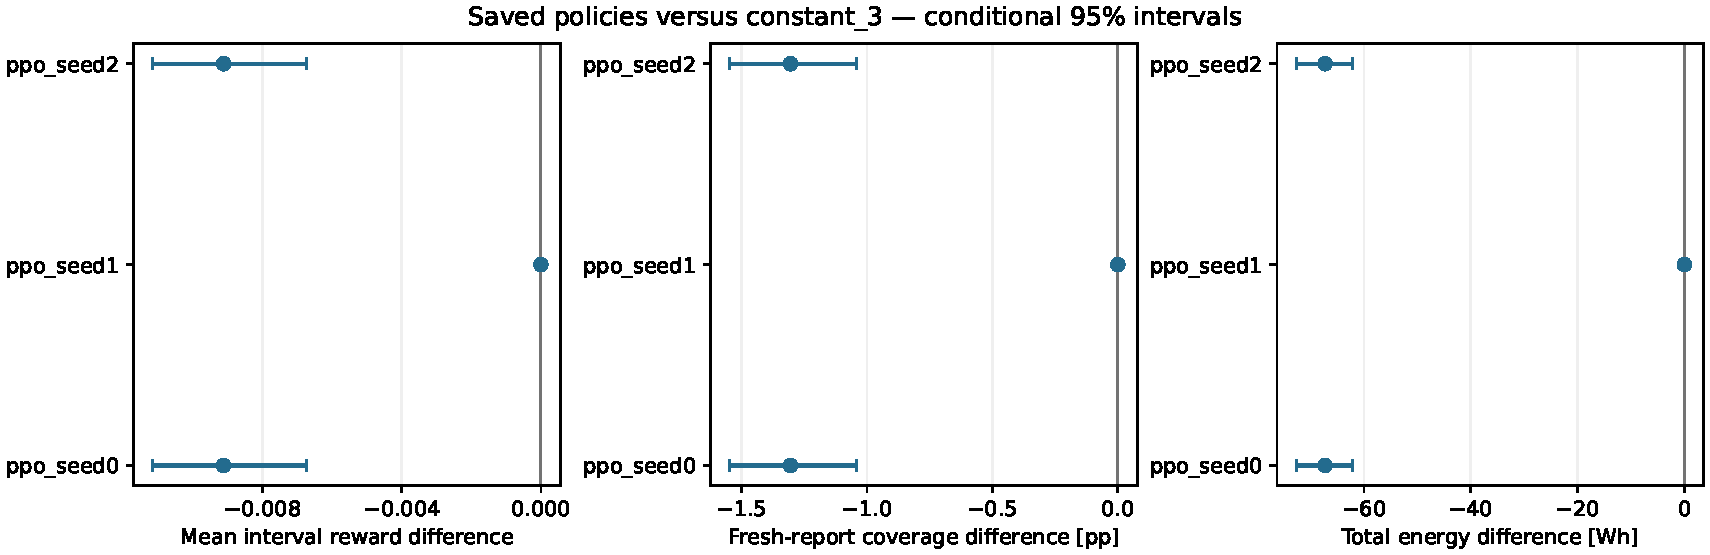
\includegraphics[width=.98\textwidth]{figures/ppo_v4.pdf}
\caption{Each short PPO training seed compared with the development-selected constant setting on the same held-out world seeds. Intervals condition on the trained policies. Favorable energy differences are negative; favorable reward and coverage differences are positive.}
\label{fig:v4ppo}\end{figure*}
The three training runs completed at 2.74--3.70 steps/s on a shared CPU. A separate 256-step, two-chunk run exercised the progress wrapper and optimizer continuation. Neither that software check nor a 2048-step pilot establishes convergence. The useful deliverable is a reproducible way to test learning against strong fixed settings, with no guarantee that extra training improves coverage or reward.
Action logs show that ppo seed0 used action 1 at every evaluated decision; ppo seed1 used action 3 at every evaluated decision; ppo seed2 used action 1 at every evaluated decision. This observed constant behavior provides no evidence of learned state-dependent adaptation, even when its score matches a strong fixed setting.


The Windows handoff adds chunked checkpoints, explicit progress, a machine-specific
runtime estimate and development/test scripts. Resuming restores PPO parameters,
optimizer and step count but restarts environment trajectories. The current continuation runner assigns a distinct, recorded environment stream to each chunk, derived from the training seed and completed step count. This prevents deliberate replay of the same initial seed sequence. Chunk boundaries
therefore change the training experiment; chunked and uninterrupted runs are not
claimed identical. The reported 2048-step pilots use one uninterrupted chunk each.
